\documentclass{article}
\setlength{\textwidth}{14cm}
\usepackage[utf8]{inputenc}
\usepackage{amsmath, amsfonts, amssymb}
\usepackage[finnish]{babel}
\usepackage{graphicx}
\graphicspath{{../images/}}
\usepackage{biblatex}
\usepackage{csquotes}
\addbibresource{viitteet.bib}
\usepackage{hyperref}
\hypersetup{
    colorlinks=true,
    linkcolor=blue,
    filecolor=green,      
    urlcolor=cyan,
    pdftitle={Neuroverkot ja koneoppiminen},
    pdfpagemode=FullScreen,
    citecolor = blue,
}



\usepackage[a4paper, left = 57pt, right = 57pt, top = 43pt, bottom = 43pt]{geometry}

\author{Joonas von Lerber}
\title{Neuroverkkojen luominen koodissa}

\begin{document}
\maketitle

\tableofcontents

\vskip15pt
\hrule
\vskip15pt

\section{Johdanto}

Keinotekoiset neuroverkot ovat koneoppimisen malleja, jotka pyrkivät karkeasti mallintamaan biologisia neuroverkkoja.
Keinotekoinen neuroverkko muodostuu monesta tekoneuronista ja tekoneuronien välisistä yhteyksistä, mitkä ovat usein
järjestetty kerroksiin. Neuroverkkojen on havaittu suoriutuvan mainiosti monista klassifikaatio- ja regressio ongelmista,
mikä tekee niistä hyödyllisiä työkaluja moneen tehtävään. Neuroverkkoja opetetaan ratkaisemaan ongelmia empiirisellä
häviön minimoinnilla\cite{vapnik1999nature}, jossa pyritään minimoimaan todellistä häviötä minimoimalla empiiristä häviötä.
Tämä tarkoittaa neuroverkkojen tapauksessa muuttelemalla neuroverkon sisäisiä parametreja kuten synapsien vahvuutta ja neuronien
herkkyyttä saadaksemme neuroverkon arvion ulostulosta lähemmäksi kouluttamisdatan antamaa oikeaa ulostuloa.

Keinotekoisten neuroverkkojen ymmärtäminen teoreettisesti on tärkeää, mutta miten neuroverkon voi luoda tietokoneella.
Miten voi itse opettaa neuroverkkoa suorittamaan ongelman ja kuinka neuroverkot rakentuvat muistissa? % Pliis tähän joku toinen kysymys :DD
Jotta neuroverkon voi rakentaa itse, täytyy ensin ymmärtää neuroverkko matemaattisena mallina, mitä käsittelen toisessa \href{http://example.com}{artikkelissani}. % Tähän sit vaikka se solmun artikkeli

\section{Rust ohjelmointikieli ja käytetyt työkalut}

Artikkelissa tulen käyttämään esimerkkikoodina ja pohjana \href {https://www.rust-lang.org/}{Rust ohjelmointikieltä}, joka on matalan tason muistiturvallinenlasjfölasjdfölasjkdfölaskjflöj,%% joo saan tän joskus valmiiks 
mutta esimerkkikoodit eivät käänny, sillä olen poistanut siitä ymmärtävyyttä haittaavia Rustin erikoisuuksia. Mikäli kääntyvää esimerkkikoodia halutaan,
voi sen löytää projektin \href{https://github.com/Joonas-vonlerber/rusticneurons}{githubista}.

\begin{figure}
    \centering
    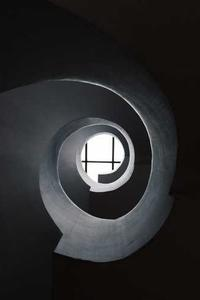
\includegraphics{testimage.jpg}
    \caption{testikuva}
    \label{testikuva}
\end{figure}

\section{Neuroverkko-tyyppi}

filler

\subsection{Neuroverkon kerros}

filler

\subsection{Neuroverkko listana kerroksia}

filler

\subsection{Neuroverkon metodit}

filler

\section{Vastavirta-algoritmi ja gradienttimenetelmä}

filler

\subsection{Vastavirta-algoritmi}

filler

\subsection{Perinteinen gradinettimenetelmä}

filler

\subsection{Optimoidut gradienttimenetelmät}

filler

\section{Tiivistelmä}

filler

\printbibliography

\end{document}